\section{继承中的类型转换}
无论对于何种继承方式,我们都可以作这样的理解:一个派生类对象当中内嵌了一个基类对象。这个基类对象只拥有基类的成员;而派生类的对象拥有基类成员在内的所有成员。在上一章的代码中,我们也反复看到了派生类对象到基类对象的隐式类型转换。那么,这个转换在什么条件下是可以的,什么条件下是禁止的?基类对象能转换为派生类对象吗?对于指针和引用来说,情况是否又会有些不同呢?这些问题的答案就在本节当中。\par
\subsection*{对象的类型转换}
在继承时,如果我们没有人为提供转换构造函数或者自定义转换函数,那么编译器就会生成一个隐式的,从派生类到基类的类型转换函数。这个类型转换函数允许派生类的对象通过 \lstinline@static_cast@ 转换为基类的对象。
\begin{lstlisting}
struct Base { /*...*/ };
struct Derived : Base { /*...*/ }; //内置了一个Derived到Base类型的转换函数
\end{lstlisting}\par
但是,这个转换函数的可见性是取决于继承方式的:
\begin{itemize}
    \item 如果 \lstinline@Derived@ 类公开继承自 \lstinline@Base@ 类,那么这个转换函数相当于是 \lstinline@Derived@ 的公有成员。
    \item 如果 \lstinline@Derived@ 类受保护继承自 \lstinline@Base@ 类,那么这个转换函数相当于是 \lstinline@Derived@ 的受保护成员。
    \item 如果 \lstinline@Derived@ 类受私有继承自 \lstinline@Base@ 类,那么这个转换函数相当于是 \lstinline@Derived@ 的私有成员。
\end{itemize}\par
对于上一章中的 \lstinline@Husky@ 类的对象来说,这个类型转换函数是 \lstinline@Husky@ 类的公有成员,所以我们可以在任何一个地方把 \lstinline@Husky@ 类的对象转换成 \lstinline@Dog@ 类。\par
而上一章中的 \lstinline@stack@ 则不同,我们只能在 \lstinline@stack@ 类当中进行类型转换;而在类之外,这个转换函数不可见,我们不能进行 \lstinline@stack@ 到 \lstinline@std::vector<int>@ 的类型转换。\par
那么,基类对象能否隐式类型转换为派生类对象呢?答案是否定的。原因也很简单:无论何种继承方式,派生类对象所需要的信息量都比基类对象更多\footnote{至少是不少于。}。也就是说,如果要把派生类对象转换为基类对象,我们不需要提供额外信息,单纯把内嵌于其中的基类对象挖出来就足够了;但如果把基类对象转换为派生类对象,我们就需要提供额外的信息,否则编译器就不知道要如何补全缺失数据。\par
所以,如果我们希望允许基类到派生类之间的类型转换,就必须自行设计转换构造函数或者自定义转换函数。还是以我们写的 \lstinline@stack@ 为例,我们就在 \lstinline@stack@ 类中定义了一个 \lstinline@explicit@ 的转换构造函数。
\begin{lstlisting}
public:
    explicit stack(const std::vector<int>&); //接收一个std::vector<int>对象
\end{lstlisting}
这样一来我们就可以用显式类型转换把基类 \lstinline@std::vector<int>@ 对象转换成派生类 \lstinline@stack@ 对象了。\par
\subsection*{指针/引用的向上类型转换}
对于指针/引用类型来说,情况会稍显复杂。\par
我们还是来想一下内存吧。对于一个派生类的对象来说,在它的内存空间中,既有属于基类的成员对象,又有属于派生类的成员对象。比如下面这段代码,作为基类成员的 \lstinline@Base::a@ 在 \lstinline@Derive@ 对象的内存空间之中拥有自己的一席之地。
\begin{lstlisting}
class Base {
    int a;
};
class Derived : public Base{
    int b;
};
int main() {
    std::cout << sizeof(Base) << ' ' << sizeof(Derived);
}
\end{lstlisting}
这段代码的运行结果如下:\\\noindent\rule{\linewidth}{.2pt}\texttt{
4 8
}\\\noindent\rule{\linewidth}{.2pt}\par
你瞧,\lstinline@Derived@ 所占用的内存空间大小为8字节,这说明它包含了 \lstinline@Base::a@ 和 \lstinline@Derived::b@ 两个成员。那么当我们对一个 \lstinline@Derived*@ 指针取内容时,程序将会取该字节起的8个字节作为一个 \lstinline@Derived@ 对象。\par
那么假如我把它转换成 \lstinline@Base*@ 指针然后取内容呢?程序只会取该字节起的4个字节作为一个 \lstinline@Base@ 对象。\par
所以我们不难发现,因为 \lstinline@Base@ 对象是内嵌在 \lstinline@Derived@ 对象当中的,我们就可以用 \lstinline@Base*@ 指针来取 \lstinline@Derived@ 对象中的基类部分,如图10.1所示。
\begin{figure}[htbp]
    \centering
    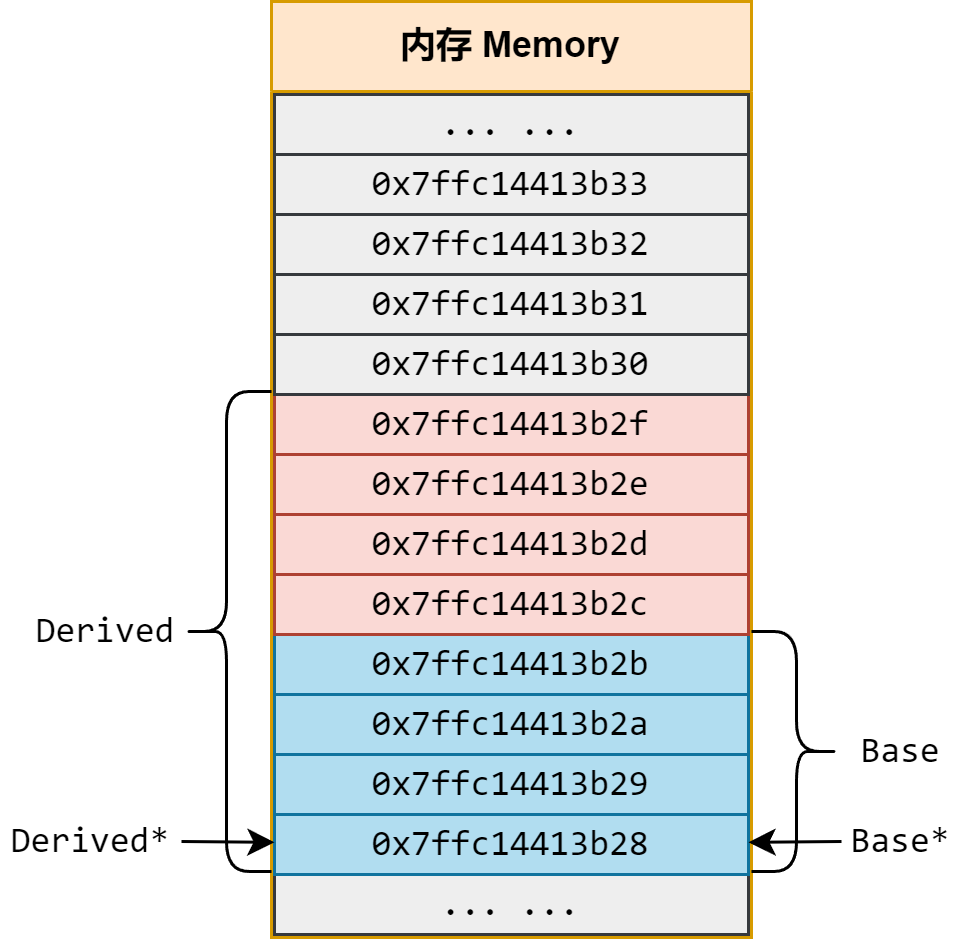
\includegraphics[width=.7\textwidth]{../images/generalized_parts/10_derived_class_object_and_subobject_in_memory.png}
    \caption{用基类指针指向内嵌于派生类中的基类对象}
\end{figure}
所以对于公有继承来说,我们可以把派生类的指针隐式类型转换为基类的指针。
\begin{lstlisting}
    Derived d {/*...*/};
    Base *b = &d; //&d被隐式类型转换为Base*类型,并赋值给b
\end{lstlisting}\par
至于私有继承和受保护继承,它们的规律和对象之间的类型转换很相似——受保护继承的派生类指针只有在派生类及``派生类的派生类''中可以转换为基类指针;私有继承的派生类指针只能在这个类中转换为基类指针。\par
无论继承权限如何,我们都把这种\textbf{派生类指针到基类指针的类型转换称为向上类型转换(Upcasting)}\footnote{我们在习惯上会把继承关系图中的基类画在上方,派生类画在下方,因此得名。}。向上类型转换总是安全的,因为基类指针访问的范围总是不大于派生类指针,所以就不会发生访问内存``越界''这样的问题。\par
引用也可以进行类型转换,道理相同:派生类的对象或者引用类型可以向上类型转换成基类的引用。所以如果我们要写一个对所有狗类都通用的函数,我们就不必为 \lstinline@Husky@, \lstinline@Retriever@ 等类型写一大堆重载,只需要写 \lstinline@Dog@ 一个类就行了。
\begin{lstlisting}
void fun(const Dog &dog) { //可以接收Dog类及其public派生类的对象
    //...
}
int main() {
    Husky mine {/*...*/};
    fun(mine); //Husky对象到Dog引用的向上类型转换
}
\end{lstlisting}\par
这里我们看到的都是指针/引用的隐式类型转换。如果要做显式类型转换的话,我们用 \lstinline@static_cast@ 来实现就可以了。\par
\subsection*{指针/引用的向下类型转换}
派生类的指针/引用可以转换为基类的引用,只要在特定继承方式下这种类型转换是可见的就行。相反地,基类的指针/引用也可以类型转换为派生类。但是相较于前者,这种基类到派生类的转换不仅多了限制,还可能存在危险。\par
基类指针/引用到派生类指针/引用的类型转换必须显式地进行——换句话说,你必须知道你正在做什么,不能稀里糊涂地就把类型转换给执行了。\par
为什么编译器要把这个功能限制地如此严格呢?这是因为,这种\textbf{基类指针/引用到派生类指针/引用的向下类型转换(Downcasting)}存在着访问越界的潜在风险。\par
\begin{figure}[htbp]
    \centering
    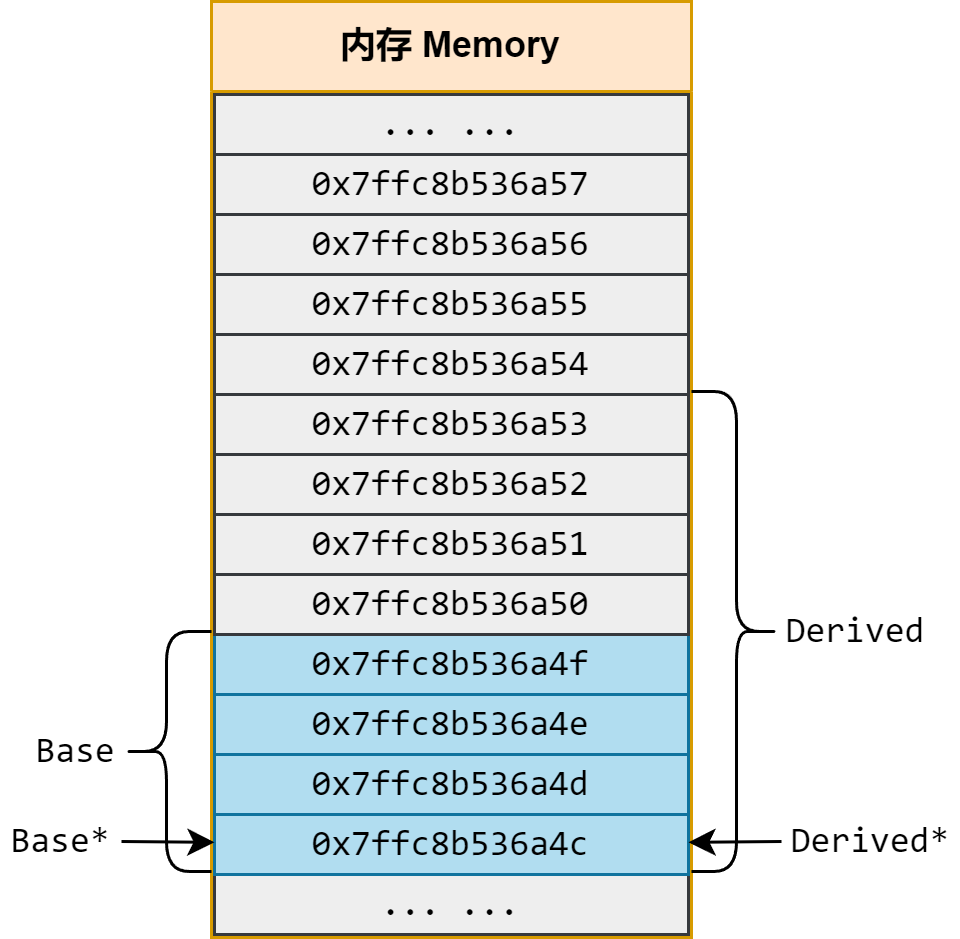
\includegraphics[width=.7\textwidth]{../images/generalized_parts/10_possible_issues_in_downcasting.png}
    \caption{用派生类指针指向基类对象,这是未定义行为}
\end{figure}
如图10.2所示,如果我们定义了一个 \lstinline@Base@ 类对象而用 \lstinline@Derived*@ 指针指向它,那么这个 \lstinline@Derived*@ 指针指向的内存范围除了这个 \lstinline@Base@ 对象以外,还有4个字节的其它空间。这4个字节可能存储了其它变量的部分信息,或者只是一些存储着杂乱无章信息的未使用空间。但夫论如何,当我们试图访问这些空间中的内容时,将会得到不确定的结果——这是一种未定义行为。\par
那么什么情况下这种类型转换是有意义的呢?只有一种情况:这个指针原本就是指向派生类对象的,只不过它出于某种原因转换成了 \lstinline@Base*@ 而已。这样一来,我们就能确保这个基类指针到派生类指针的转换是安全的。但另一个问题在于,当我们拿到一个基类指针时,我们怎么才能知道这个基类指针到底是不是原本指向派生类对象的呢?很遗憾,因为指针的指向是可以任意改变的,所以我们不能在编译时确定它是不是指向派生类对象的。\par
\lstinline@static_cast@ 的解决方法是不解决——它只是死板地执行类型转换的操作而已,至于这里潜在的风险,它是不会管的。也正因如此,在向下类型转换的过程中,我们再使用 \lstinline@static_cast@ 已经不合适,必须寻求一种能在运行时判断类型并给出相应转换结果的方案,这就是动态类型转换 \lstinline@dynamic_cast@。\par
动态类型转换可以保证程序能够安全地进行向下类型转换。当我们试图把基类指针转换为派生类指针时,程序会进行运行时检查:如果这个基类指针是指向派生类的,那么它可以成功地进行类型转换;否则,这个类型转换只能返回一个 \lstinline@nullptr@。当我们试图把基类引用转换为派生类引用时,程序会进行运行时检查:如果这个基类引用是对派生类对象的引用\footnote{其本质说白了还是指针的指向。引用都是靠指针来实现的。},那么它可以成功地进行类型转换;否则,就会抛出 \lstinline@std::bad_cast@ 异常\footnote{我们会在第十二章中讲解异常。}。\par
\lstinline@dynamic_cast@ 的用法和 \lstinline@static_cast@ 非常相仿,但是我们先别急着用它。动态类型转换要求基类比须是多态的——接下来的一节马上就来讲解这个问题。\par
